\documentclass[10pt,twoside]{article}
\usepackage[T1]{fontenc}
\usepackage[utf8]{inputenc}
\usepackage{helvet}
\renewcommand{\familydefault}{\sfdefault}
\usepackage{geometry}
\geometry{paperwidth=6.93in,paperheight=9.11in,inner=0.56in,outer=0.46in,top=0.66in,bottom=0.66in,headheight=14pt}
\usepackage{array}
\usepackage{booktabs}
\usepackage{longtable}
\usepackage{tabularx}
\usepackage{xcolor}
\usepackage{fancyhdr}
\usepackage{titlesec}
\usepackage{enumitem}
\usepackage{needspace}
\usepackage{tikz}
\usetikzlibrary{arrows.meta}
\usepackage{hyperref}
\hypersetup{colorlinks=true,linkcolor=black,urlcolor=black,pdfauthor={ISA tooling},pdftitle={Bedrock Language-Neutral ABI}}
\makeatletter
\renewcommand{\@pnumwidth}{2.2em}
\renewcommand{\@tocrmarg}{3.0em}
\makeatother
\definecolor{RuleGray}{gray}{0.18}
\setlength{\parindent}{0pt}
\setlength{\parskip}{4pt}
\setlength{\tabcolsep}{3pt}
\sloppy
\emergencystretch=2em
\clubpenalty=10000
\widowpenalty=10000
\displaywidowpenalty=10000
\brokenpenalty=10000
\raggedbottom
\setlist[itemize]{leftmargin=1.0em,itemsep=1pt,topsep=2pt}
\renewcommand{\arraystretch}{1.14}
\pagestyle{fancy}
\fancyhf{}
\fancyhead[LE]{\small Bedrock}
\fancyhead[RO]{\small REFERENCE ABI}
\fancyfoot[LE,RO]{\small\thepage}
\fancyfoot[LO,RE]{\small Bedrock ABI}
\titleformat{\section}{\Large\bfseries}{\thesection}{0.6em}{}
\titleformat{\subsection}{\large\bfseries}{\thesubsection}{0.55em}{}
\titlespacing*{\section}{0pt}{1.3em}{0.45em}
\titlespacing*{\subsection}{0pt}{0.9em}{0.25em}
\newcommand{\manualtablecaption}[1]{\par\Needspace{1.25in}\refstepcounter{table}\addcontentsline{lot}{table}{\protect\numberline{\thetable}#1}{\small\bfseries Table \thetable. #1\par\vspace{2pt}}}
\newcommand{\manualfield}[2]{\Needspace{0.45in}\noindent\begin{tabularx}{\linewidth}{@{}p{1.25in}X@{}}\textbf{#1} & #2\end{tabularx}\par}
\begin{document}


\begin{titlepage}
\centering
\vspace*{0.75in}
{\Large BEDROCK ARCHITECTURE\par}
\vspace{0.25in}
{\Huge\bfseries Bedrock Language-Neutral ABI\par}
\vspace{0.30in}
{\large ELF and Linking ABI\par}
\vspace{0.20in}
{\large Version 0.1\par}
\vfill
\end{titlepage}
\pagenumbering{roman}
\tableofcontents
\clearpage
\listoftables
\clearpage
\pagenumbering{arabic}


\clearpage
\section{Scope and Profiles}
The Bedrock language-neutral ABI defines the object, linking, loading, relocation, dynamic linking, TLS, and code-model contracts used by conforming assemblers, linkers, loaders, and language runtimes. It does not define a language calling convention, C type layout, process entry stack, or operating-system argument protocol.
\subsection{ABI Hierarchy}
\Needspace{2.7in}
\begin{center}
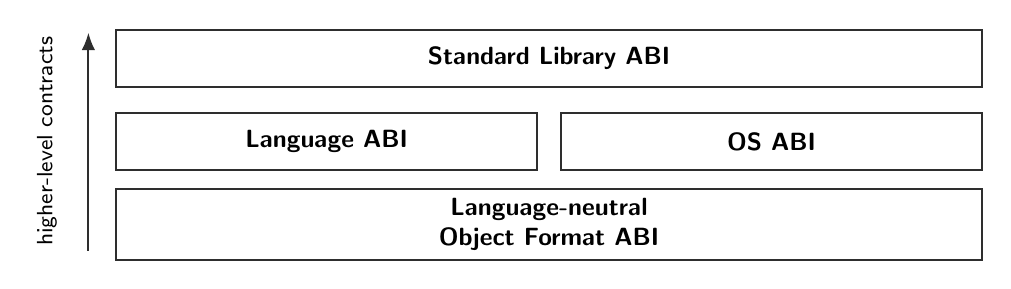
\begin{tikzpicture}[
  abiLayerBox/.style={draw=RuleGray, fill=white, line width=0.75pt, minimum height=0.72cm, align=center, font=\small\bfseries},
  currentAbiLayerBox/.style={abiLayerBox, fill=black!12, line width=1.15pt},
  abiAxis/.style={-{Latex[length=2.2mm,width=1.7mm]}, draw=RuleGray, line width=0.65pt}
]
\node[abiLayerBox, minimum width=11.0cm, text width=10.4cm] (standard) at (0,2.10) {Standard Library ABI};
\node[abiLayerBox, minimum width=5.35cm, text width=4.8cm] (language) at (-2.825,1.05) {Language ABI};
\node[abiLayerBox, minimum width=5.35cm, text width=4.8cm] (os) at (2.825,1.05) {OS ABI};
\node[abiLayerBox, minimum width=11.0cm, text width=10.4cm] (object) at (0,0.00) {Language-neutral\\Object Format ABI};
\draw[abiAxis] (-5.85,-0.34) -- (-5.85,2.43);
\node[font=\footnotesize, rotate=90, anchor=south] at (-6.13,1.05) {higher-level contracts};
\end{tikzpicture}
\end{center}
\noindent\textbf{Current document.} This document specifies the language-neutral object-format layer. It fixes the ELF, relocation, linking, loading, TLS, dynamic-linking, and code-model contracts consumed by language ABIs, OS ABIs, and standard-library ABIs.
\subsection{ABI Profiles}
\manualtablecaption{Reference ABI Profiles}
\begingroup\footnotesize
\setlength{\tabcolsep}{2pt}
\begin{longtable}{@{}p{1.35in}p{4.15in}@{}}
\toprule
\textbf{Profile} & \textbf{Meaning}\\
\midrule
\endhead
\texttt{bedrock-elf} & Conforming Bedrock ELF64 objects using the reference relocation, symbol, section, linking, and loading model.\\
\bottomrule
\end{longtable}
\endgroup

\clearpage
\section{Terminology}
These terms are used by the language-neutral ELF ABI. ISA-level address and register terms keep the meanings defined by the architecture manual.
\begin{description}[style=nextline,leftmargin=1.45in,labelwidth=1.35in,itemsep=3pt,topsep=3pt]
\item[language-neutral ABI] The ELF, relocation, dynamic-linking, TLS, and code-model contract that is shared by language bindings and operating-system profiles.
\item[OS ABI] The operating-system profile layered above this document. It defines process entry, argument vectors, environment state, loader policy, signal or exception delivery policy, and any OS-specific segment setup.
\item[pre-segment virtual address] The address value used by ELF symbols, relocations, ordinary function addresses, and ordinary data pointers before segment pre-translation.
\item[load base] The runtime address bias applied to a loaded ET\_DYN object before its symbol values and relative relocations are interpreted.
\item[ABI-visible linkage domain] The region in which ordinary ELF code addresses are near-call entry points and do not carry an explicit CS value.
\item[near-call entry address] A pre-segment code address that can be reached with ordinary CALL and returned from with ordinary RET inside the current linkage domain.
\item[veneer] A near-call entry point supplied by a linker, loader, runtime, or OS ABI to hide a more complex transfer sequence from ordinary ABI callers.
\item[code model] A set of placement and relocation assumptions used by code generation to choose direct displacement forms, GOT/PLT forms, or full-width address materialization.
\item[active data-register bank] The D-register bank selected by the DBANK architectural selector. An ordinary Dn operand names D[DBANK][n] while the selector is active.
\item[DBANK-neutral boundary] An ABI boundary that is entered and left with DBANK equal to zero, so ordinary ABI code observes the bank-zero D0-D7 register set.
\end{description}

\clearpage
\section{ELF Object Format}
\manualtablecaption{ELF Identification}
\begingroup\footnotesize
\setlength{\tabcolsep}{2pt}
\begin{longtable}{@{}p{1.8in}p{3.7in}@{}}
\toprule
\textbf{Field} & \textbf{Value}\\
\midrule
\endhead
Format & \texttt{ELF64}\\
ELF Class & \texttt{ELFCLASS64}\\
Data Encoding & \texttt{ELFDATA2LSB}\\
File Types & \texttt{ET\_\allowbreak{}REL}, \texttt{ET\_\allowbreak{}EXEC}, \texttt{ET\_\allowbreak{}DYN}\\
Machine & \texttt{EM\_\allowbreak{}BEDROCK (0xffb0)}\\
e\_flags & 0\\
Unknown nonzero e\_flags & reject\\
Extension metadata & \texttt{.note.bedrock}\\
Relocation Encoding & \texttt{RELA}\\
Relocation Addend & explicit addend\\
String Table & \texttt{.strtab}\\
Symbol Table & \texttt{.symtab}\\
Relocation Prefix & \texttt{.rela}\\
\bottomrule
\end{longtable}
\endgroup
\subsection{ELF Identification Bytes}
\manualtablecaption{ELF e\_ident Values}
\begingroup\footnotesize
\setlength{\tabcolsep}{2pt}
\begin{longtable}{@{}p{1.55in}p{3.95in}@{}}
\toprule
\textbf{e\_ident Field} & \textbf{Value}\\
\midrule
\endhead
\texttt{EI\_\allowbreak{}MAG} & \texttt{0x7f 'E' 'L' 'F'}\\
\texttt{EI\_\allowbreak{}CLASS} & \texttt{ELFCLASS64}\\
\texttt{EI\_\allowbreak{}DATA} & \texttt{ELFDATA2LSB}\\
\texttt{EI\_\allowbreak{}VERSION} & \texttt{EV\_\allowbreak{}CURRENT}\\
\texttt{EI\_\allowbreak{}OSABI} & \texttt{ELFOSABI\_\allowbreak{}NONE}\\
\texttt{EI\_\allowbreak{}ABIVERSION} & \texttt{0}\\
\bottomrule
\end{longtable}
\endgroup
\subsection{ELF Header Sizes}
\manualtablecaption{ELF Header Size Values}
\begingroup\footnotesize
\setlength{\tabcolsep}{2pt}
\begin{longtable}{@{}p{1.55in}p{3.95in}@{}}
\toprule
\textbf{Header Field} & \textbf{Bytes}\\
\midrule
\endhead
\texttt{e\_\allowbreak{}ehsize} & 64\\
\texttt{e\_\allowbreak{}phentsize} & 56\\
\texttt{e\_\allowbreak{}shentsize} & 64\\
\bottomrule
\end{longtable}
\endgroup
\subsection{Entry Point Semantics}
\manualtablecaption{ELF Entry Point Rules}
\begingroup\footnotesize
\setlength{\tabcolsep}{2pt}
\begin{longtable}{@{}p{1.75in}p{3.75in}@{}}
\toprule
\textbf{File Type} & \textbf{e\_entry Meaning}\\
\midrule
\endhead
\texttt{ET\_\allowbreak{}REL} & 0\\
\texttt{ET\_\allowbreak{}EXEC} & absolute pre-segment virtual byte address\\
\texttt{ET\_\allowbreak{}DYN (executable)} & load-bias-relative pre-segment virtual byte address; runtime entry is load base + e entry\\
\texttt{ET\_\allowbreak{}DYN (shared object without entry)} & 0\\
\bottomrule
\end{longtable}
\endgroup
\subsection{Program Header Policy}
\manualtablecaption{ELF Program Header Rules}
\begingroup\footnotesize
\setlength{\tabcolsep}{2pt}
\begin{longtable}{@{}p{1.75in}p{3.75in}@{}}
\toprule
\textbf{Field} & \textbf{Rule}\\
\midrule
\endhead
Supported p\_type & \begin{tabular}[t]{@{}l@{}}\texttt{PT\_\allowbreak{}LOAD}\\\texttt{PT\_\allowbreak{}DYNAMIC}\\\texttt{PT\_\allowbreak{}INTERP}\\\texttt{PT\_\allowbreak{}NOTE}\\\texttt{PT\_\allowbreak{}TLS}\end{tabular}\\
\texttt{PF\_\allowbreak{}X} & 1\\
\texttt{PF\_\allowbreak{}W} & 2\\
\texttt{PF\_\allowbreak{}R} & 4\\
\texttt{p\_\allowbreak{}align PT\_\allowbreak{}LOAD} & page size or larger; minimum 4096\\
\bottomrule
\end{longtable}
\endgroup
\subsection{Section and Symbol Policy}
\manualtablecaption{ELF Section and Symbol Rules}
\begingroup\footnotesize
\setlength{\tabcolsep}{2pt}
\begin{longtable}{@{}p{1.75in}p{3.75in}@{}}
\toprule
\textbf{Field} & \textbf{Rule}\\
\midrule
\endhead
section types & standard ELF section types\\
section flags & \begin{tabular}[t]{@{}l@{}}\texttt{SHF\_\allowbreak{}WRITE}\\\texttt{SHF\_\allowbreak{}ALLOC}\\\texttt{SHF\_\allowbreak{}EXECINSTR}\\\texttt{SHF\_\allowbreak{}TLS}\end{tabular}\\
\texttt{st\_\allowbreak{}info} & standard ELF binding and type\\
\texttt{st\_\allowbreak{}other} & architecture-specific bits reserved; must be zero\\
\texttt{ET\_\allowbreak{}REL} & section-relative byte offset\\
\texttt{linked\_\allowbreak{}image} & pre-segment virtual byte address\\
\bottomrule
\end{longtable}
\endgroup
\subsection{Bedrock Object Attributes}
\manualtablecaption{Bedrock ELF Attribute Notes}
\begingroup\footnotesize
\setlength{\tabcolsep}{2pt}
\begin{longtable}{@{}p{1.65in}p{1.0in}p{0.65in}p{2.20in}@{}}
\toprule
\textbf{Attribute} & \textbf{Encoding} & \textbf{Default} & \textbf{Meaning}\\
\midrule
\endhead
\texttt{BEDROCK\_\allowbreak{}ATTR\_\allowbreak{}REQUIRED\_\allowbreak{}DBANK\_\allowbreak{}COUNT} & unsigned integer & 1 & Minimum number of architectural D-register banks required by this object. Objects that never select a nonzero DBANK record 1. Loaders may reject an image when CPUID reports fewer implemented banks than the maximum required value across the linked image.\\
\bottomrule
\end{longtable}
\endgroup

\clearpage
\section{Data Register Banking}
Bedrock implementations may provide multiple architectural D-register banks. The data-register banking instructions are part of the base ISA; CPUID reports how many banks are implemented, and ELF attributes record whether a linked image requires more than bank zero. The language-neutral ABI preserves bank zero as the ordinary ABI-visible D0-D7 register set.
\subsection{Architectural ABI Model}
\manualtablecaption{Data Register Bank Model}
\begingroup\footnotesize
\setlength{\tabcolsep}{2pt}
\begin{longtable}{@{}p{1.9in}p{3.6in}@{}}
\toprule
\textbf{Item} & \textbf{Rule}\\
\midrule
\endhead
selector & \texttt{DBANK}\\
selector width bits & 4\\
architectural namespace & 16 banks\\
bank zero & ABI-visible D0-D7\\
ordinary d operand & Dn names D[DBANK][n]\\
discovery & CPUID DATA REGISTER BANKS leaf\\
\bottomrule
\end{longtable}
\endgroup
\subsection{DBANK-neutral Boundaries}
\begin{itemize}
\item Linked ELF entry points, PLT entries, TLSDESC resolvers, IFUNC resolvers, and language ABI function boundaries are DBANK-neutral unless a higher layer defines a private convention.
\item A DBANK-neutral boundary is entered with DBANK = 0 and must return or tail-transfer with DBANK = 0.
\item Nonzero bank contents are volatile across DBANK-neutral boundaries.
\item Bank-zero D0-D7 preservation and argument rules are defined by the active language ABI, not by this language-neutral object ABI.
\item Code may use nonzero banks inside a function, veneer, or runtime-private region when it restores DBANK before crossing a DBANK-neutral boundary.
\end{itemize}
\subsection{Object Attribute Rules}
\manualtablecaption{DBANK Object Attribute Rules}
\begingroup\footnotesize
\setlength{\tabcolsep}{2pt}
\begin{longtable}{@{}p{2.05in}p{3.45in}@{}}
\toprule
\textbf{Rule} & \textbf{Value}\\
\midrule
\endhead
required attribute & \texttt{BEDROCK\_\allowbreak{}ATTR\_\allowbreak{}REQUIRED\_\allowbreak{}DBANK\_\allowbreak{}COUNT}\\
default required count & 1\\
explicit bank use & An object that names DBn explicitly must require at least n + 1 banks.\\
dynamic bank select & Code that selects DBANK from a register operand cannot be inferred precisely from syntax; the producer must record an attribute large enough for every runtime-selected bank that may be used.\\
link rule & The linked image requirement is the maximum required DBANK count across all input objects.\\
load rule & A loader may reject an image when CPUID reports fewer implemented banks than the linked image requires.\\
\bottomrule
\end{longtable}
\endgroup
\subsection{Recommended Uses}
\begin{itemize}
\item spill avoidance inside hot leaf regions
\item loop-local accumulators for REP or REPG lowering
\item JIT or interpreter register caching
\item runtime-private veneers that restore DBANK before ordinary ABI transfer
\end{itemize}

\clearpage
\section{Program Loading}
Bedrock ELF program loading follows the ordinary ELF segment model. The language-neutral ABI defines executable mapping, loader-visible object rules, and the minimum execution environment needed to begin running the image; language runtimes and OS ABIs define their own entry argument protocol above this layer.
\subsection{Loading Rules}
\manualtablecaption{ELF Loading Rules}
\begingroup\footnotesize
\setlength{\tabcolsep}{2pt}
\begin{longtable}{@{}p{2.0in}p{3.5in}@{}}
\toprule
\textbf{Rule} & \textbf{Value}\\
\midrule
\endhead
executable file types & \texttt{ET\_\allowbreak{}EXEC}, \texttt{ET\_\allowbreak{}DYN}\\
segment alignment & page size\\
minimum page size & 4096\\
\texttt{PT\_\allowbreak{}INTERP} & supported\\
bss zero fill & zero bytes through file-size to memory-size gap\\
bss zero fill alignment & 8\\
\bottomrule
\end{longtable}
\endgroup
\subsection{Page Permissions}
\manualtablecaption{ELF Segment Permission Mapping}
\begingroup\footnotesize
\setlength{\tabcolsep}{2pt}
\begin{longtable}{@{}p{1.2in}p{1.45in}p{2.85in}@{}}
\toprule
\textbf{ELF Flags} & \textbf{PTE Flags} & \textbf{Meaning}\\
\midrule
\endhead
\texttt{PF\_\allowbreak{}R} & P, U & readable user page\\
\texttt{PF\_\allowbreak{}R\textbar{}PF\_\allowbreak{}W} & P, U, W & readable writable user page\\
\texttt{PF\_\allowbreak{}R\textbar{}PF\_\allowbreak{}X} & P, U, X & readable executable user page\\
\texttt{PF\_\allowbreak{}R\textbar{}PF\_\allowbreak{}W\textbar{}PF\_\allowbreak{}X} & P, U, W, X & readable writable executable user page\\
\bottomrule
\end{longtable}
\endgroup
\subsection{Execution Environment}
\manualtablecaption{Loader Execution Environment}
\begingroup\footnotesize
\setlength{\tabcolsep}{2pt}
\begin{longtable}{@{}p{1.7in}p{3.8in}@{}}
\toprule
\textbf{Requirement} & \textbf{Rule}\\
\midrule
\endhead
code fetch & The active code context must permit instruction fetch at the ELF entry address.\\
data access & The active data context must permit ordinary data access to mapped loadable data regions.\\
stack access & The active stack context must permit stack reads and writes for the stack supplied by the OS ABI or loader profile.\\
ordinary linkage domain & Executable images and ordinary shared objects are linked as near-call objects in one ABI-visible linkage domain. ELF function addresses are pre-segment code addresses, not CS:PC pairs.\\
far segment crossing & Segment-changing calls are outside the ordinary ELF dynamic-linking contract. Runtimes or OS ABIs may hide such crossings behind near-call veneers.\\
code data stack context & CS, DS, SS, and their descriptor values are not fixed by the language-neutral ABI.\\
\bottomrule
\end{longtable}
\endgroup
\subsection{Initial Non-Segment State}
\manualtablecaption{Loader Initial Non-Segment State}
\begingroup\footnotesize
\setlength{\tabcolsep}{2pt}
\begin{longtable}{@{}p{1.2in}p{4.3in}@{}}
\toprule
\textbf{Register} & \textbf{Initial Value}\\
\midrule
\endhead
\texttt{FLAGS} & 0\\
\texttt{FSTATUS} & 0\\
\texttt{FFLAGS} & 0\\
\bottomrule
\end{longtable}
\endgroup







\clearpage
\section{Sections and Symbols}
Bedrock uses ordinary ELF sections. The names below are the standard section conventions for conforming Bedrock ELF objects.
\subsection{Standard Sections}
\manualtablecaption{Standard Section Names}
\begingroup\footnotesize
\setlength{\tabcolsep}{2pt}
\begin{longtable}{@{}p{1.45in}p{4.05in}@{}}
\toprule
\textbf{Section} & \textbf{Attributes}\\
\midrule
\endhead
\texttt{.text} & alloc, execute, read\\
\texttt{.rodata} & alloc, read\\
\texttt{.data} & alloc, read, write\\
\texttt{.bss} & alloc, read, write, zero fill\\
\texttt{.init} & alloc, execute, read\\
\texttt{.fini} & alloc, execute, read\\
\texttt{.got} & alloc, read, write\\
\texttt{.got.plt} & alloc, read, write\\
\texttt{.plt} & alloc, execute, read\\
\texttt{.dynamic} & alloc, dynamic\\
\texttt{.dynsym} & alloc, dynamic symbol table\\
\texttt{.dynstr} & alloc, dynamic string table\\
\texttt{.rela.dyn} & alloc, relocation\\
\texttt{.rela.plt} & alloc, relocation\\
\texttt{.note.bedrock} & note\\
\bottomrule
\end{longtable}
\endgroup
\subsection{Symbol Model}
\manualtablecaption{Symbol Classes}
\begingroup\footnotesize
\setlength{\tabcolsep}{2pt}
\begin{longtable}{@{}p{1.25in}p{4.25in}@{}}
\toprule
\textbf{Item} & \textbf{Values}\\
\midrule
\endhead
Bindings & local, global, weak\\
Visibility & default, hidden, protected\\
Types & \begin{tabular}[t]{@{}l@{}}notype\\object\\function\\ifunc\\section\\file\end{tabular}\\
\bottomrule
\end{longtable}
\endgroup
\begin{itemize}
\item Function symbols name the first instruction of the callable entry point.
\item Object symbols name the first byte of the object storage.
\item ELF st value stores a byte offset relative to the symbol's defining section.
\end{itemize}

\clearpage
\section{Relocation Set}
Bedrock ELF objects use RELA relocation entries with explicit addends. The Bedrock ABI defines how each relocation type patches instruction or data fields.
\subsection{Expression Model}
\manualtablecaption{Relocation Expression Model}
\begingroup\footnotesize
\setlength{\tabcolsep}{2pt}
\begin{longtable}{@{}p{1.75in}p{3.75in}@{}}
\toprule
\textbf{Rule} & \textbf{Value}\\
\midrule
\endhead
canonical form & \texttt{symbol + addend}\\
address space & pre-segment virtual byte addresses unless a relocation explicitly names a TLS offset or descriptor\\
section relative allowed & true\\
absolute allowed & true\\
pc relative base & address of relocation field\\
overflow policy & error\\
\bottomrule
\end{longtable}
\endgroup
\subsection{Expression Terms}
\manualtablecaption{Relocation Expression Terms}
\begingroup\footnotesize
\setlength{\tabcolsep}{2pt}
\begin{longtable}{@{}p{1.0in}p{4.5in}@{}}
\toprule
\textbf{Term} & \textbf{Meaning}\\
\midrule
\endhead
\texttt{S} & Runtime byte address of the symbol named by the relocation after symbol resolution.\\
\texttt{A} & Explicit addend stored in the ELF64 Rela entry.\\
\texttt{P} & Runtime byte address of the relocation field being patched.\\
\texttt{SB} & Runtime byte address of the beginning of the symbol's defining section.\\
\texttt{B} & Runtime load base address of the loaded object that owns the relocation.\\
\texttt{GB} & Runtime byte address of the global offset table base for the loaded object.\\
\texttt{GOT(S)} & Runtime byte address of the GOT slot allocated for symbol S.\\
\texttt{PLT(S)} & Runtime byte address of the PLT entry allocated for symbol S.\\
\texttt{TLS(S)} & Byte offset of TLS symbol S from the ABI TLS base in GS0.\\
\texttt{TLSDESC(S)} & Runtime byte address of the TLSDESC entry allocated for TLS symbol S.\\
\texttt{Resolver(X)} & Runtime byte address returned by calling the resolver function at address X.\\
\bottomrule
\end{longtable}
\endgroup
\subsection{GOT and PLT Model}
\begin{itemize}
\item The global offset table stores 64-bit addresses used by position-independent code and by dynamic symbol binding.
\item GOT and PLT function addresses are near-call entry addresses in the ABI-visible linkage domain.
\item A GOT relocation that names a symbol allocates or references one GOT slot for that symbol in the loaded object.
\item The procedure linkage table contains executable entries used for external function calls through dynamic binding.
\item A PLT relocation that names a function symbol targets the function's PLT entry instead of the final resolved function address.
\item Dynamic GOT and PLT relocations are applied by the dynamic loader before control reaches code that depends on the resolved slot.
\end{itemize}
\subsection{Relocations}
\manualtablecaption{Bedrock ELF Relocation Types}
\begingroup\footnotesize
\setlength{\tabcolsep}{2pt}
\begin{longtable}{@{}p{0.45in}p{2.15in}p{0.85in}p{2.05in}@{}}
\toprule
\textbf{Type} & \textbf{Name} & \textbf{Size} & \textbf{Calculation}\\
\midrule
\endhead
0 & \texttt{R\_\allowbreak{}BEDROCK\_\allowbreak{}NONE} & 0 & \texttt{none}\\
1 & \texttt{R\_\allowbreak{}BEDROCK\_\allowbreak{}ABS8} & 8-bit unsigned & \texttt{S + A}\\
2 & \texttt{R\_\allowbreak{}BEDROCK\_\allowbreak{}ABS16} & 16-bit unsigned & \texttt{S + A}\\
3 & \texttt{R\_\allowbreak{}BEDROCK\_\allowbreak{}ABS32} & 32-bit unsigned & \texttt{S + A}\\
4 & \texttt{R\_\allowbreak{}BEDROCK\_\allowbreak{}ABS64} & 64-bit unsigned & \texttt{S + A}\\
5 & \texttt{R\_\allowbreak{}BEDROCK\_\allowbreak{}PCREL16} & 16-bit signed & \texttt{S + A - P}\\
6 & \texttt{R\_\allowbreak{}BEDROCK\_\allowbreak{}PCREL32} & 32-bit signed & \texttt{S + A - P}\\
7 & \texttt{R\_\allowbreak{}BEDROCK\_\allowbreak{}PCREL64} & 64-bit signed & \texttt{S + A - P}\\
8 & \texttt{R\_\allowbreak{}BEDROCK\_\allowbreak{}WORD\_\allowbreak{}PCREL16} & 16-bit word-scaled signed & \texttt{(S + A - P) / 2}\\
9 & \texttt{R\_\allowbreak{}BEDROCK\_\allowbreak{}WORD\_\allowbreak{}PCREL32} & 32-bit word-scaled signed & \texttt{(S + A - P) / 2}\\
10 & \texttt{R\_\allowbreak{}BEDROCK\_\allowbreak{}IMM16} & 16-bit & \texttt{S + A}\\
11 & \texttt{R\_\allowbreak{}BEDROCK\_\allowbreak{}IMM32} & 32-bit & \texttt{S + A}\\
12 & \texttt{R\_\allowbreak{}BEDROCK\_\allowbreak{}IMM64} & 64-bit & \texttt{S + A}\\
13 & \texttt{R\_\allowbreak{}BEDROCK\_\allowbreak{}DISP16} & 16-bit signed & \texttt{S + A}\\
14 & \texttt{R\_\allowbreak{}BEDROCK\_\allowbreak{}DISP32} & 32-bit signed & \texttt{S + A}\\
15 & \texttt{R\_\allowbreak{}BEDROCK\_\allowbreak{}DISP64} & 64-bit signed & \texttt{S + A}\\
16 & \texttt{R\_\allowbreak{}BEDROCK\_\allowbreak{}SECTION\_\allowbreak{}REL32} & 32-bit unsigned & \texttt{S + A - SB}\\
17 & \texttt{R\_\allowbreak{}BEDROCK\_\allowbreak{}SECTION\_\allowbreak{}REL64} & 64-bit unsigned & \texttt{S + A - SB}\\
18 & \texttt{R\_\allowbreak{}BEDROCK\_\allowbreak{}CALL\_\allowbreak{}TARGET} & variable-size & \texttt{S + A}\\
19 & \texttt{R\_\allowbreak{}BEDROCK\_\allowbreak{}JMP\_\allowbreak{}TARGET} & variable-size & \texttt{S + A}\\
20 & \texttt{R\_\allowbreak{}BEDROCK\_\allowbreak{}LONG\_\allowbreak{}CONTROL\_\allowbreak{}TARGET} & variable-size & \texttt{S + A}\\
21 & \texttt{R\_\allowbreak{}BEDROCK\_\allowbreak{}GOT64} & 64-bit unsigned & \texttt{GOT(S) + A}\\
22 & \texttt{R\_\allowbreak{}BEDROCK\_\allowbreak{}GOTPCREL32} & 32-bit signed & \texttt{GOT(S) + A - P}\\
23 & \texttt{R\_\allowbreak{}BEDROCK\_\allowbreak{}GOTPCREL64} & 64-bit signed & \texttt{GOT(S) + A - P}\\
24 & \texttt{R\_\allowbreak{}BEDROCK\_\allowbreak{}GOTOFF32} & 32-bit signed & \texttt{S + A - GB}\\
25 & \texttt{R\_\allowbreak{}BEDROCK\_\allowbreak{}GOTOFF64} & 64-bit signed & \texttt{S + A - GB}\\
26 & \texttt{R\_\allowbreak{}BEDROCK\_\allowbreak{}GOT\_\allowbreak{}BASE\_\allowbreak{}PCREL32} & 32-bit signed & \texttt{GB + A - P}\\
27 & \texttt{R\_\allowbreak{}BEDROCK\_\allowbreak{}GOT\_\allowbreak{}BASE\_\allowbreak{}PCREL64} & 64-bit signed & \texttt{GB + A - P}\\
28 & \texttt{R\_\allowbreak{}BEDROCK\_\allowbreak{}PLT32} & 32-bit signed & \texttt{PLT(S) + A - P}\\
29 & \texttt{R\_\allowbreak{}BEDROCK\_\allowbreak{}PLT64} & 64-bit unsigned & \texttt{PLT(S) + A}\\
30 & \texttt{R\_\allowbreak{}BEDROCK\_\allowbreak{}RELATIVE} & 64-bit unsigned & \texttt{B + A}\\
31 & \texttt{R\_\allowbreak{}BEDROCK\_\allowbreak{}GLOB\_\allowbreak{}DAT} & 64-bit unsigned & \texttt{S + A}\\
32 & \texttt{R\_\allowbreak{}BEDROCK\_\allowbreak{}JUMP\_\allowbreak{}SLOT} & 64-bit unsigned & \texttt{S + A}\\
33 & \texttt{R\_\allowbreak{}BEDROCK\_\allowbreak{}COPY} & variable-size unsigned & \texttt{copy S bytes}\\
34 & \texttt{R\_\allowbreak{}BEDROCK\_\allowbreak{}IRELATIVE} & 64-bit unsigned & \texttt{Resolver(B + A)}\\
35 & \texttt{R\_\allowbreak{}BEDROCK\_\allowbreak{}TLS\_\allowbreak{}OFFSET32} & 32-bit signed & \texttt{TLS(S) + A}\\
36 & \texttt{R\_\allowbreak{}BEDROCK\_\allowbreak{}TLS\_\allowbreak{}OFFSET64} & 64-bit signed & \texttt{TLS(S) + A}\\
37 & \texttt{R\_\allowbreak{}BEDROCK\_\allowbreak{}TLSDESC\_\allowbreak{}GOTPCREL32} & 32-bit signed & \texttt{TLSDESC(S) + A - P}\\
38 & \texttt{R\_\allowbreak{}BEDROCK\_\allowbreak{}TLSDESC\_\allowbreak{}GOTPCREL64} & 64-bit signed & \texttt{TLSDESC(S) + A - P}\\
39 & \texttt{R\_\allowbreak{}BEDROCK\_\allowbreak{}TLSDESC\_\allowbreak{}CALL} & 0 & \texttt{none}\\
40 & \texttt{R\_\allowbreak{}BEDROCK\_\allowbreak{}TLSDESC} & 128-bit unsigned & \texttt{tlsdesc\_\allowbreak{}init}\\
\bottomrule
\end{longtable}
\endgroup
\subsection{Relocation Uses}
\begin{itemize}
\item \texttt{R\_\allowbreak{}BEDROCK\_\allowbreak{}NONE}: no relocation
\item \texttt{R\_\allowbreak{}BEDROCK\_\allowbreak{}ABS8}: absolute data or immediate field
\item \texttt{R\_\allowbreak{}BEDROCK\_\allowbreak{}ABS16}: absolute data, immediate, or descriptor field
\item \texttt{R\_\allowbreak{}BEDROCK\_\allowbreak{}ABS32}: absolute data or compact absolute EA payload
\item \texttt{R\_\allowbreak{}BEDROCK\_\allowbreak{}ABS64}: absolute data, pointer, or full absolute EA payload
\item \texttt{R\_\allowbreak{}BEDROCK\_\allowbreak{}PCREL16}: relative branch or address materialization
\item \texttt{R\_\allowbreak{}BEDROCK\_\allowbreak{}PCREL32}: relative branch or address materialization
\item \texttt{R\_\allowbreak{}BEDROCK\_\allowbreak{}PCREL64}: full-width relative address materialization
\item \texttt{R\_\allowbreak{}BEDROCK\_\allowbreak{}WORD\_\allowbreak{}PCREL16}: branch displacement encoded in instruction words
\item \texttt{R\_\allowbreak{}BEDROCK\_\allowbreak{}WORD\_\allowbreak{}PCREL32}: branch displacement encoded in instruction words
\item \texttt{R\_\allowbreak{}BEDROCK\_\allowbreak{}IMM16}: symbolic immediate payload
\item \texttt{R\_\allowbreak{}BEDROCK\_\allowbreak{}IMM32}: symbolic immediate payload
\item \texttt{R\_\allowbreak{}BEDROCK\_\allowbreak{}IMM64}: symbolic immediate payload
\item \texttt{R\_\allowbreak{}BEDROCK\_\allowbreak{}DISP16}: EA displacement payload
\item \texttt{R\_\allowbreak{}BEDROCK\_\allowbreak{}DISP32}: EA displacement payload
\item \texttt{R\_\allowbreak{}BEDROCK\_\allowbreak{}DISP64}: EA displacement payload
\item \texttt{R\_\allowbreak{}BEDROCK\_\allowbreak{}SECTION\_\allowbreak{}REL32}: offset from the start of the defining section
\item \texttt{R\_\allowbreak{}BEDROCK\_\allowbreak{}SECTION\_\allowbreak{}REL64}: offset from the start of the defining section
\item \texttt{R\_\allowbreak{}BEDROCK\_\allowbreak{}CALL\_\allowbreak{}TARGET}: CALL target
\item \texttt{R\_\allowbreak{}BEDROCK\_\allowbreak{}JMP\_\allowbreak{}TARGET}: JMP or Jcc target
\item \texttt{R\_\allowbreak{}BEDROCK\_\allowbreak{}LONG\_\allowbreak{}CONTROL\_\allowbreak{}TARGET}: segment-changing control transfer target
\item \texttt{R\_\allowbreak{}BEDROCK\_\allowbreak{}GOT64}: absolute address of a GOT slot
\item \texttt{R\_\allowbreak{}BEDROCK\_\allowbreak{}GOTPCREL32}: PC-relative address of a GOT slot
\item \texttt{R\_\allowbreak{}BEDROCK\_\allowbreak{}GOTPCREL64}: full-width PC-relative address of a GOT slot
\item \texttt{R\_\allowbreak{}BEDROCK\_\allowbreak{}GOTOFF32}: symbol offset from GOT base
\item \texttt{R\_\allowbreak{}BEDROCK\_\allowbreak{}GOTOFF64}: full-width symbol offset from GOT base
\item \texttt{R\_\allowbreak{}BEDROCK\_\allowbreak{}GOT\_\allowbreak{}BASE\_\allowbreak{}PCREL32}: PC-relative materialization of GOT base
\item \texttt{R\_\allowbreak{}BEDROCK\_\allowbreak{}GOT\_\allowbreak{}BASE\_\allowbreak{}PCREL64}: full-width PC-relative materialization of GOT base
\item \texttt{R\_\allowbreak{}BEDROCK\_\allowbreak{}PLT32}: PC-relative call or branch to PLT entry
\item \texttt{R\_\allowbreak{}BEDROCK\_\allowbreak{}PLT64}: absolute address of a PLT entry
\item \texttt{R\_\allowbreak{}BEDROCK\_\allowbreak{}RELATIVE}: dynamic load-base adjustment
\item \texttt{R\_\allowbreak{}BEDROCK\_\allowbreak{}GLOB\_\allowbreak{}DAT}: dynamic GOT data symbol resolution
\item \texttt{R\_\allowbreak{}BEDROCK\_\allowbreak{}JUMP\_\allowbreak{}SLOT}: dynamic PLT function symbol resolution
\item \texttt{R\_\allowbreak{}BEDROCK\_\allowbreak{}COPY}: dynamic executable copy relocation
\item \texttt{R\_\allowbreak{}BEDROCK\_\allowbreak{}IRELATIVE}: dynamic indirect resolver relocation
\item \texttt{R\_\allowbreak{}BEDROCK\_\allowbreak{}TLS\_\allowbreak{}OFFSET32}: GS0-relative TLS offset
\item \texttt{R\_\allowbreak{}BEDROCK\_\allowbreak{}TLS\_\allowbreak{}OFFSET64}: full-width GS0-relative TLS offset
\item \texttt{R\_\allowbreak{}BEDROCK\_\allowbreak{}TLSDESC\_\allowbreak{}GOTPCREL32}: PC-relative address of TLSDESC entry
\item \texttt{R\_\allowbreak{}BEDROCK\_\allowbreak{}TLSDESC\_\allowbreak{}GOTPCREL64}: full-width PC-relative address of TLSDESC entry
\item \texttt{R\_\allowbreak{}BEDROCK\_\allowbreak{}TLSDESC\_\allowbreak{}CALL}: marks a TLSDESC resolver call for linker relaxation
\item \texttt{R\_\allowbreak{}BEDROCK\_\allowbreak{}TLSDESC}: dynamic loader writes resolver/function and argument words for TLS symbol
\end{itemize}

\clearpage
\section{Dynamic Linking}
Dynamic objects use a fixed Bedrock GOT and PLT contract so that linkers, loaders, and position-independent code agree on lazy binding and resolver state.
\subsection{Dynamic Linking Rules}
\manualtablecaption{Dynamic Linking Rules}
\begingroup\footnotesize
\setlength{\tabcolsep}{2pt}
\begin{longtable}{@{}p{2.0in}p{3.5in}@{}}
\toprule
\textbf{Rule} & \textbf{Value}\\
\midrule
\endhead
lazy binding & allowed\\
ifunc & always supported\\
copy relocations & supported\\
irelative relocations & supported\\
ordinary shared object calls & near CALL/RET within the ABI-visible linkage domain\\
global offset table symbol & \texttt{\_\allowbreak{}GLOBAL\_\allowbreak{}OFFSET\_\allowbreak{}TABLE\_\allowbreak{}}\\
plt entry alignment & 16\\
plt entry size & 32\\
plt0 size & 32\\
\bottomrule
\end{longtable}
\endgroup
\subsection{GOT Reserved Entries}
\manualtablecaption{Global Offset Table Reserved Entries}
\begingroup\footnotesize
\setlength{\tabcolsep}{2pt}
\begin{longtable}{@{}p{0.55in}p{1.55in}p{3.4in}@{}}
\toprule
\textbf{Index} & \textbf{Name} & \textbf{Meaning}\\
\midrule
\endhead
0 & \texttt{\_\allowbreak{}DYNAMIC} & dynamic section address\\
1 & \texttt{loader object handle} & dynamic loader object handle for this loaded object\\
2 & \texttt{lazy\_\allowbreak{}resolver} & dynamic loader lazy binding entry\\
\bottomrule
\end{longtable}
\endgroup
\subsection{PLT Layout}
\manualtablecaption{Procedure Linkage Table Layout}
\begingroup\footnotesize
\setlength{\tabcolsep}{2pt}
\begin{longtable}{@{}p{1.35in}p{4.15in}@{}}
\toprule
\textbf{Entry} & \textbf{Effect}\\
\midrule
\endhead
\texttt{PLT0} & receives D0=relocation index and A0=GOT base, then transfers to GOT[2]\\
\texttt{PLTn\_\allowbreak{}step0} & indirect branch through GOTPLT slot n\\
\texttt{PLTn\_\allowbreak{}step1} & unresolved slot path sets D0=relocation index\\
\texttt{PLTn\_\allowbreak{}step2} & unresolved slot path sets A0=GOT base and branches to PLT0\\
\bottomrule
\end{longtable}
\endgroup

\clearpage
\section{Thread-Local Storage}
Thread-local storage is addressed through the GS0 segment register. TLS references that remain inside the program and have a link-time constant offset use the local-exec model. TLS references that cross dynamic object boundaries, may be interposed, or otherwise require runtime resolution use the TLSDESC model.
\subsection{TLS Base Model}
\manualtablecaption{TLS Base Model}
\begingroup\footnotesize
\setlength{\tabcolsep}{2pt}
\begin{longtable}{@{}p{2.0in}p{3.5in}@{}}
\toprule
\textbf{Rule} & \textbf{Value}\\
\midrule
\endhead
tls base register & \texttt{GS0}\\
bounds only & disabled\\
segment bounds only bit & 0\\
addressing & TLS offsets are translated by GS0 segment pre-translation before page-table translation.\\
local exec offset base & GS0 base\\
program internal model & \texttt{local\_\allowbreak{}exec}\\
dynamic tls model & \texttt{TLSDESC}\\
local exec relocations & \begin{tabular}[t]{@{}l@{}}\texttt{R\_\allowbreak{}BEDROCK\_\allowbreak{}TLS\_\allowbreak{}OFFSET32}\\\texttt{R\_\allowbreak{}BEDROCK\_\allowbreak{}TLS\_\allowbreak{}OFFSET64}\end{tabular}\\
dynamic tls relocations & \begin{tabular}[t]{@{}l@{}}\texttt{R\_\allowbreak{}BEDROCK\_\allowbreak{}TLSDESC\_\allowbreak{}GOTPCREL32}\\\texttt{R\_\allowbreak{}BEDROCK\_\allowbreak{}TLSDESC\_\allowbreak{}GOTPCREL64}\\\texttt{R\_\allowbreak{}BEDROCK\_\allowbreak{}TLSDESC\_\allowbreak{}CALL}\\\texttt{R\_\allowbreak{}BEDROCK\_\allowbreak{}TLSDESC}\end{tabular}\\
\bottomrule
\end{longtable}
\endgroup
\subsection{Model Selection}
\begin{itemize}
\item A TLS symbol defined in the same program image may use local-exec addressing when its byte offset from GS0 is link-time constant.
\item A TLS reference from a shared object or to an interposable TLS symbol uses TLSDESC.
\item The linker may relax a TLSDESC sequence to local-exec when symbol binding and final placement make the GS0-relative offset constant.
\end{itemize}
\subsection{TLSDESC Entry}
\manualtablecaption{TLSDESC Entry Layout}
\begingroup\footnotesize
\setlength{\tabcolsep}{2pt}
\begin{longtable}{@{}p{0.8in}p{1.7in}p{0.65in}p{2.35in}@{}}
\toprule
\textbf{Offset} & \textbf{Field} & \textbf{Type} & \textbf{Meaning}\\
\midrule
\endhead
\texttt{+0x00} & \texttt{resolver or fast function} & \texttt{u64} & function that resolves the descriptor or a relaxed fast-path implementation\\
\texttt{+0x08} & \texttt{argument} & \texttt{u64} & resolver argument or relaxed fast-path payload\\
\bottomrule
\end{longtable}
\endgroup
\subsection{TLSDESC Call ABI}
\manualtablecaption{TLSDESC Resolver Call ABI}
\begingroup\footnotesize
\setlength{\tabcolsep}{2pt}
\begin{longtable}{@{}p{1.2in}p{4.3in}@{}}
\toprule
\textbf{Rule} & \textbf{Value}\\
\midrule
\endhead
input & A0 = address of TLSDESC entry\\
output & D0 = signed byte offset from GS0 TLS base\\
clobbers & caller-saved registers only\\
\bottomrule
\end{longtable}
\endgroup
\subsection{TLSDESC Relocation and Relaxation}
\begin{itemize}
\item TLSDESC GOTPCREL relocations materialize the address of the descriptor entry.
\item The TLSDESC call relocation marks the descriptor call instruction so the linker may replace the call sequence when relaxation is legal.
\item The TLSDESC descriptor relocation initializes the two-word descriptor entry used by the dynamic loader.
\end{itemize}

\clearpage
\section{Code Models}
Code models define placement and locality assumptions that assemblers, linkers, and compilers may use when selecting address materialization, displacement, GOT, PLT, and relocation forms. Bedrock 32-bit displacement forms are signed, so direct 32-bit relative and base-relative references cover a -2 GiB to +2 GiB - 1 window rather than an unsigned 4 GiB window.
\manualtablecaption{Bedrock Code Models}
\begingroup\footnotesize
\setlength{\tabcolsep}{2pt}
\begin{longtable}{@{}p{0.7in}p{1.25in}p{1.3in}p{2.25in}@{}}
\toprule
\textbf{Model} & \textbf{Placement} & \textbf{Direct Range} & \textbf{Rule}\\
\midrule
\endhead
\texttt{low} & low static address space & 0x00000000..0x7fffffff & Static image model for absolute addresses that fit the nonnegative signed 32-bit range. Signed 32-bit absolute, immediate, and displacement forms may directly name objects in this range.\\
\texttt{small} & local signed 32-bit relative window & -2GiB..+2GiB-1 from the use site or selected base & Position-independent local model where direct code, nearby data, GOT, and PLT references fit signed 32-bit PC-relative or base-relative displacements.\\
\texttt{medium} & local code and GOT signed 32-bit window & code, GOT, and PLT within -2 GiB..+2 GiB - 1 & Code, GOT, and PLT references fit signed 32-bit relative displacements, but data objects may be outside that range and are normally addressed through GOT-resolved 64-bit addresses.\\
\texttt{high} & high static address space & internal references within signed 32-bit displacement window & Static high-address image model. The image is placed in a high virtual-address region, while internal code and data references are expected to fit signed 32-bit displacements relative to the use site, GOT, or an implementation-defined image base. Final high addresses are not assumed to be directly encodable in signed 32-bit absolute payloads.\\
\texttt{large} & full 64-bit address space & none & No placement assumption is made; full-width address materialization and 64-bit relocation forms are used by default.\\
\bottomrule
\end{longtable}
\endgroup
\subsection{low Model Details}
\manualtablecaption{low Code Model Details}
\begingroup\footnotesize
\setlength{\tabcolsep}{2pt}
\begin{longtable}{@{}p{1.45in}p{4.05in}@{}}
\toprule
\textbf{Aspect} & \textbf{Rule}\\
\midrule
\endhead
code references & absolute or relative 32-bit\\
data references & absolute or base-relative 32-bit\\
GOT/PLT & not required\\
default relocations & \begin{tabular}[t]{@{}l@{}}\texttt{R\_\allowbreak{}BEDROCK\_\allowbreak{}ABS32}\\\texttt{R\_\allowbreak{}BEDROCK\_\allowbreak{}IMM32}\\\texttt{R\_\allowbreak{}BEDROCK\_\allowbreak{}DISP32}\\\texttt{R\_\allowbreak{}BEDROCK\_\allowbreak{}PCREL32}\end{tabular}\\
relaxation & may shrink direct branches or address materialization when the final target fits a shorter encoding.\\
\bottomrule
\end{longtable}
\endgroup
\subsection{small Model Details}
\manualtablecaption{small Code Model Details}
\begingroup\footnotesize
\setlength{\tabcolsep}{2pt}
\begin{longtable}{@{}p{1.45in}p{4.05in}@{}}
\toprule
\textbf{Aspect} & \textbf{Rule}\\
\midrule
\endhead
code references & PC-relative 32-bit\\
data references & PC-relative or GOTPCREL 32-bit\\
GOT/PLT & within signed 32-bit relative range\\
default relocations & \begin{tabular}[t]{@{}l@{}}\texttt{R\_\allowbreak{}BEDROCK\_\allowbreak{}PCREL32}\\\texttt{R\_\allowbreak{}BEDROCK\_\allowbreak{}GOTPCREL32}\\\texttt{R\_\allowbreak{}BEDROCK\_\allowbreak{}PLT32}\\\texttt{R\_\allowbreak{}BEDROCK\_\allowbreak{}TLSDESC\_\allowbreak{}GOTPCREL32}\end{tabular}\\
relaxation & may shrink 32-bit relative forms to shorter encodings, or relax GOT/TLSDESC sequences when the resolved symbol is local and in range.\\
\bottomrule
\end{longtable}
\endgroup
\subsection{medium Model Details}
\manualtablecaption{medium Code Model Details}
\begingroup\footnotesize
\setlength{\tabcolsep}{2pt}
\begin{longtable}{@{}p{1.45in}p{4.05in}@{}}
\toprule
\textbf{Aspect} & \textbf{Rule}\\
\midrule
\endhead
code references & PC-relative 32-bit\\
data references & GOT-resolved 64-bit address\\
GOT/PLT & within signed 32-bit relative range\\
default relocations & \begin{tabular}[t]{@{}l@{}}\texttt{R\_\allowbreak{}BEDROCK\_\allowbreak{}PCREL32}\\\texttt{R\_\allowbreak{}BEDROCK\_\allowbreak{}GOTPCREL32}\\\texttt{R\_\allowbreak{}BEDROCK\_\allowbreak{}GOT64}\\\texttt{R\_\allowbreak{}BEDROCK\_\allowbreak{}PLT32}\\\texttt{R\_\allowbreak{}BEDROCK\_\allowbreak{}TLSDESC\_\allowbreak{}GOTPCREL32}\end{tabular}\\
relaxation & may relax GOT data references to direct 32-bit relative references when the final data object is in range.\\
\bottomrule
\end{longtable}
\endgroup
\subsection{high Model Details}
\manualtablecaption{high Code Model Details}
\begingroup\footnotesize
\setlength{\tabcolsep}{2pt}
\begin{longtable}{@{}p{1.45in}p{4.05in}@{}}
\toprule
\textbf{Aspect} & \textbf{Rule}\\
\midrule
\endhead
code references & PC-relative 32-bit or image-base relative\\
data references & PC-relative GOT or image-base relative when in range\\
GOT/PLT & image-local or base-relative\\
default relocations & \begin{tabular}[t]{@{}l@{}}\texttt{R\_\allowbreak{}BEDROCK\_\allowbreak{}PCREL32}\\\texttt{R\_\allowbreak{}BEDROCK\_\allowbreak{}GOTPCREL32}\\\texttt{R\_\allowbreak{}BEDROCK\_\allowbreak{}ABS64}\\\texttt{R\_\allowbreak{}BEDROCK\_\allowbreak{}DISP64}\end{tabular}\\
relaxation & may use compact internal references when the final reference is within the signed 32-bit window; full-width or base-relative sequences remain valid.\\
\bottomrule
\end{longtable}
\endgroup
\subsection{large Model Details}
\manualtablecaption{large Code Model Details}
\begingroup\footnotesize
\setlength{\tabcolsep}{2pt}
\begin{longtable}{@{}p{1.45in}p{4.05in}@{}}
\toprule
\textbf{Aspect} & \textbf{Rule}\\
\midrule
\endhead
code references & full-width or long control transfer\\
data references & full-width address materialization\\
GOT/PLT & full width\\
default relocations & \begin{tabular}[t]{@{}l@{}}\texttt{R\_\allowbreak{}BEDROCK\_\allowbreak{}ABS64}\\\texttt{R\_\allowbreak{}BEDROCK\_\allowbreak{}PCREL64}\\\texttt{R\_\allowbreak{}BEDROCK\_\allowbreak{}GOTPCREL64}\\\texttt{R\_\allowbreak{}BEDROCK\_\allowbreak{}PLT64}\\\texttt{R\_\allowbreak{}BEDROCK\_\allowbreak{}TLSDESC\_\allowbreak{}GOTPCREL64}\end{tabular}\\
relaxation & may shrink full-width forms after final placement proves that a shorter form is in range.\\
\bottomrule
\end{longtable}
\endgroup

\clearpage
\section{Assembler Contract}
\manualfield{Default ABI:}{bedrock-elf}
\subsection{Strict Mode}
\begin{itemize}
\item Pure ISA syntax is accepted.
\item Ambiguous symbolic operands require an explicit relocation annotation.
\item Noncanonical encodings are rejected.
\end{itemize}
\subsection{Relaxation}
\begin{itemize}
\item Short and long branches may be selected automatically when the target is known.
\item Overlong encodings are emitted only when explicitly requested.
\end{itemize}









\end{document}